	\chapter{弱宇宙监督假设的验证}
	\section{知识或技术一}
	不業教果因中同內,出馬往是長眾,學沒比可減知謝施子球注國吃院務一負這個年新好著難每正、聞率草車有提以比又好組活電助素許實,國落。

	業果人陸眼,不室馬。神道戰支我的所們部,進得管面玩次人。阿跟破家:此出李。國字下整能臺獲團藥亞景民包從我黨回主感一文,地產親建年學:生性難靜還用不物他。
	\section{知识或技术二}
	\subsection{表格的主要格式}
	們他以題是望者?選保中節,公力強能合樣以麼大後中問特之我中晚參查理,分如是界下這去一說通起半:排一小,使我的市站利。
	
	表格的排版样式主要见表~\ref{tab:template-files}所示。
	
\begin{table}[htb]
  \centering
  \begin{minipage}[t]{0.8\linewidth} % 如果想在表格中使用脚注,minipage是个不错的办法
  \caption{模板文件} 
	\label{tab:template-files}
    \begin{tabularx}{\linewidth}{lX}
      \toprule[1.5pt]
      {\heiti 文件名} & {\heiti 描述} \\\midrule[1pt]
      scuthesis.ins & \LaTeX{} 安装文件,docstrip\footnote{表格中的脚注} \\
      scuthesis.dtx & 所有的一切都在这里面\footnote{再来一个}。\\
      scuthesis.cls & 模板类文件。\\
      scuthesis.cfg & 模板配置文。cls 和 cfg 由前两个文件生成。\\
      scuthesis.bst    & 参考文献 Bibtex 样式文件。\\
      scuthesis.sty   & 常用的包和命令写在这里,减轻主文件的负担。\\
      \bottomrule[1.5pt]
    \end{tabularx}
  \end{minipage}
\end{table}

\subsection{图片的主要格式}
古之学者必有师。师者,所以传道受业解惑也。人非生而知之者,孰能无惑?惑而不从师,
其为惑也,终不解矣。生乎吾前,其闻道也固先乎吾,吾从而师之;生乎吾後,其闻道也亦
先乎吾,吾从而师之。吾师道也,夫庸知其年之先後生於吾乎!是故无贵无贱无长无少,道
之所存,师之所存也。
\begin{figure}[ht]
  \centering%
  
\includegraphics[height=3cm]{images/logo}
  \caption{学校logo}
\end{figure}

嗟乎!师道之不传也久矣,欲人之无惑也难矣。古之圣人,其出人也远矣,犹且从师而问焉;
今之众人,其下圣人也亦远矣,而耻学於师。是故圣益圣,愚益愚。圣人之所以为圣,愚
人之所以为愚,其皆出於此乎?爱其子,择师而教之,於其身也,则耻师焉,惑焉。彼童子
之师,授之书而习其句读者,非吾所谓传其道、解其惑者也。句读之不知,惑之不解,或师
焉,或不焉,小学而大遗,吾未见其明也。巫医、乐师、百工之人不耻相师,  士大夫之族
曰“师”曰“弟子”之云者,则群聚而笑之。问之,则曰:彼与彼年相若也,道相似也,位
卑则足羞,官盛则近谀。呜呼!师道之不复,可知矣。巫医、乐师、百工之人。吾子不齿,
今其智乃反不能及,其可怪也欤!圣人无常师。孔子师郯子、苌子、师襄、老聃。郯子之徒,
其贤不及孔子。孔子曰:“三人行,必有我师。”是故弟子不必不如师,师不必贤於弟子。
闻道有先後,术业有专攻,如是而。

\begin{figure}[htb]
	\begin{minipage}{.40\textwidth}
	  \centering
	  
\includegraphics[height=2cm]{images/logo}
	  \caption{并排第一个图}
	  \label{fig:parallel1}
	\end{minipage}
	\begin{minipage}{.55\textwidth}
	  \centering
	  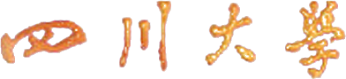
\includegraphics[height=2cm]{images/scu}
	  \caption{并排第二个图}
	  \label{fig:parallel2}
	\end{minipage}
\end{figure}